\documentclass[dvipdfmx,a4j]{jsarticle}
\usepackage[dvipdfmx]{graphicx}

\usepackage{amssymb, amsmath}
\usepackage{bm}
\usepackage{url}
\usepackage[version=3]{mhchem}
\usepackage{physics}
\usepackage{siunitx}

\usepackage[hang,small,bf]{caption}
\usepackage[subrefformat=parens]{subcaption}
\captionsetup{compatibility=false}

\usepackage{longtable}
\usepackage{newtxtext,newtxmath}

\usepackage{tabularx}

\usepackage{lscape}



\begin{document}

\section{電装系システム概要}

本機に搭載するバルブシステムの電装は、ロケット搭載基板および地上GSE電装から構成される。ロケット搭載基板の役割は、メインバルブを制御することである。また、地上GSEの役割は、GSEを制御すること、および点火操作に合わせてロケット搭載基板と通信を行い、ロケット搭載基板を制御することである。

両者はフライトピンによって締結され、ロケットの離床と同時に切断される。

\subsection{ロケット搭載基板}

ロケット搭載基板のシステムチャートを図\ref{newGenPropulsionBRDChart} に示す。

\begin{figure}[htbp]
    \centering
    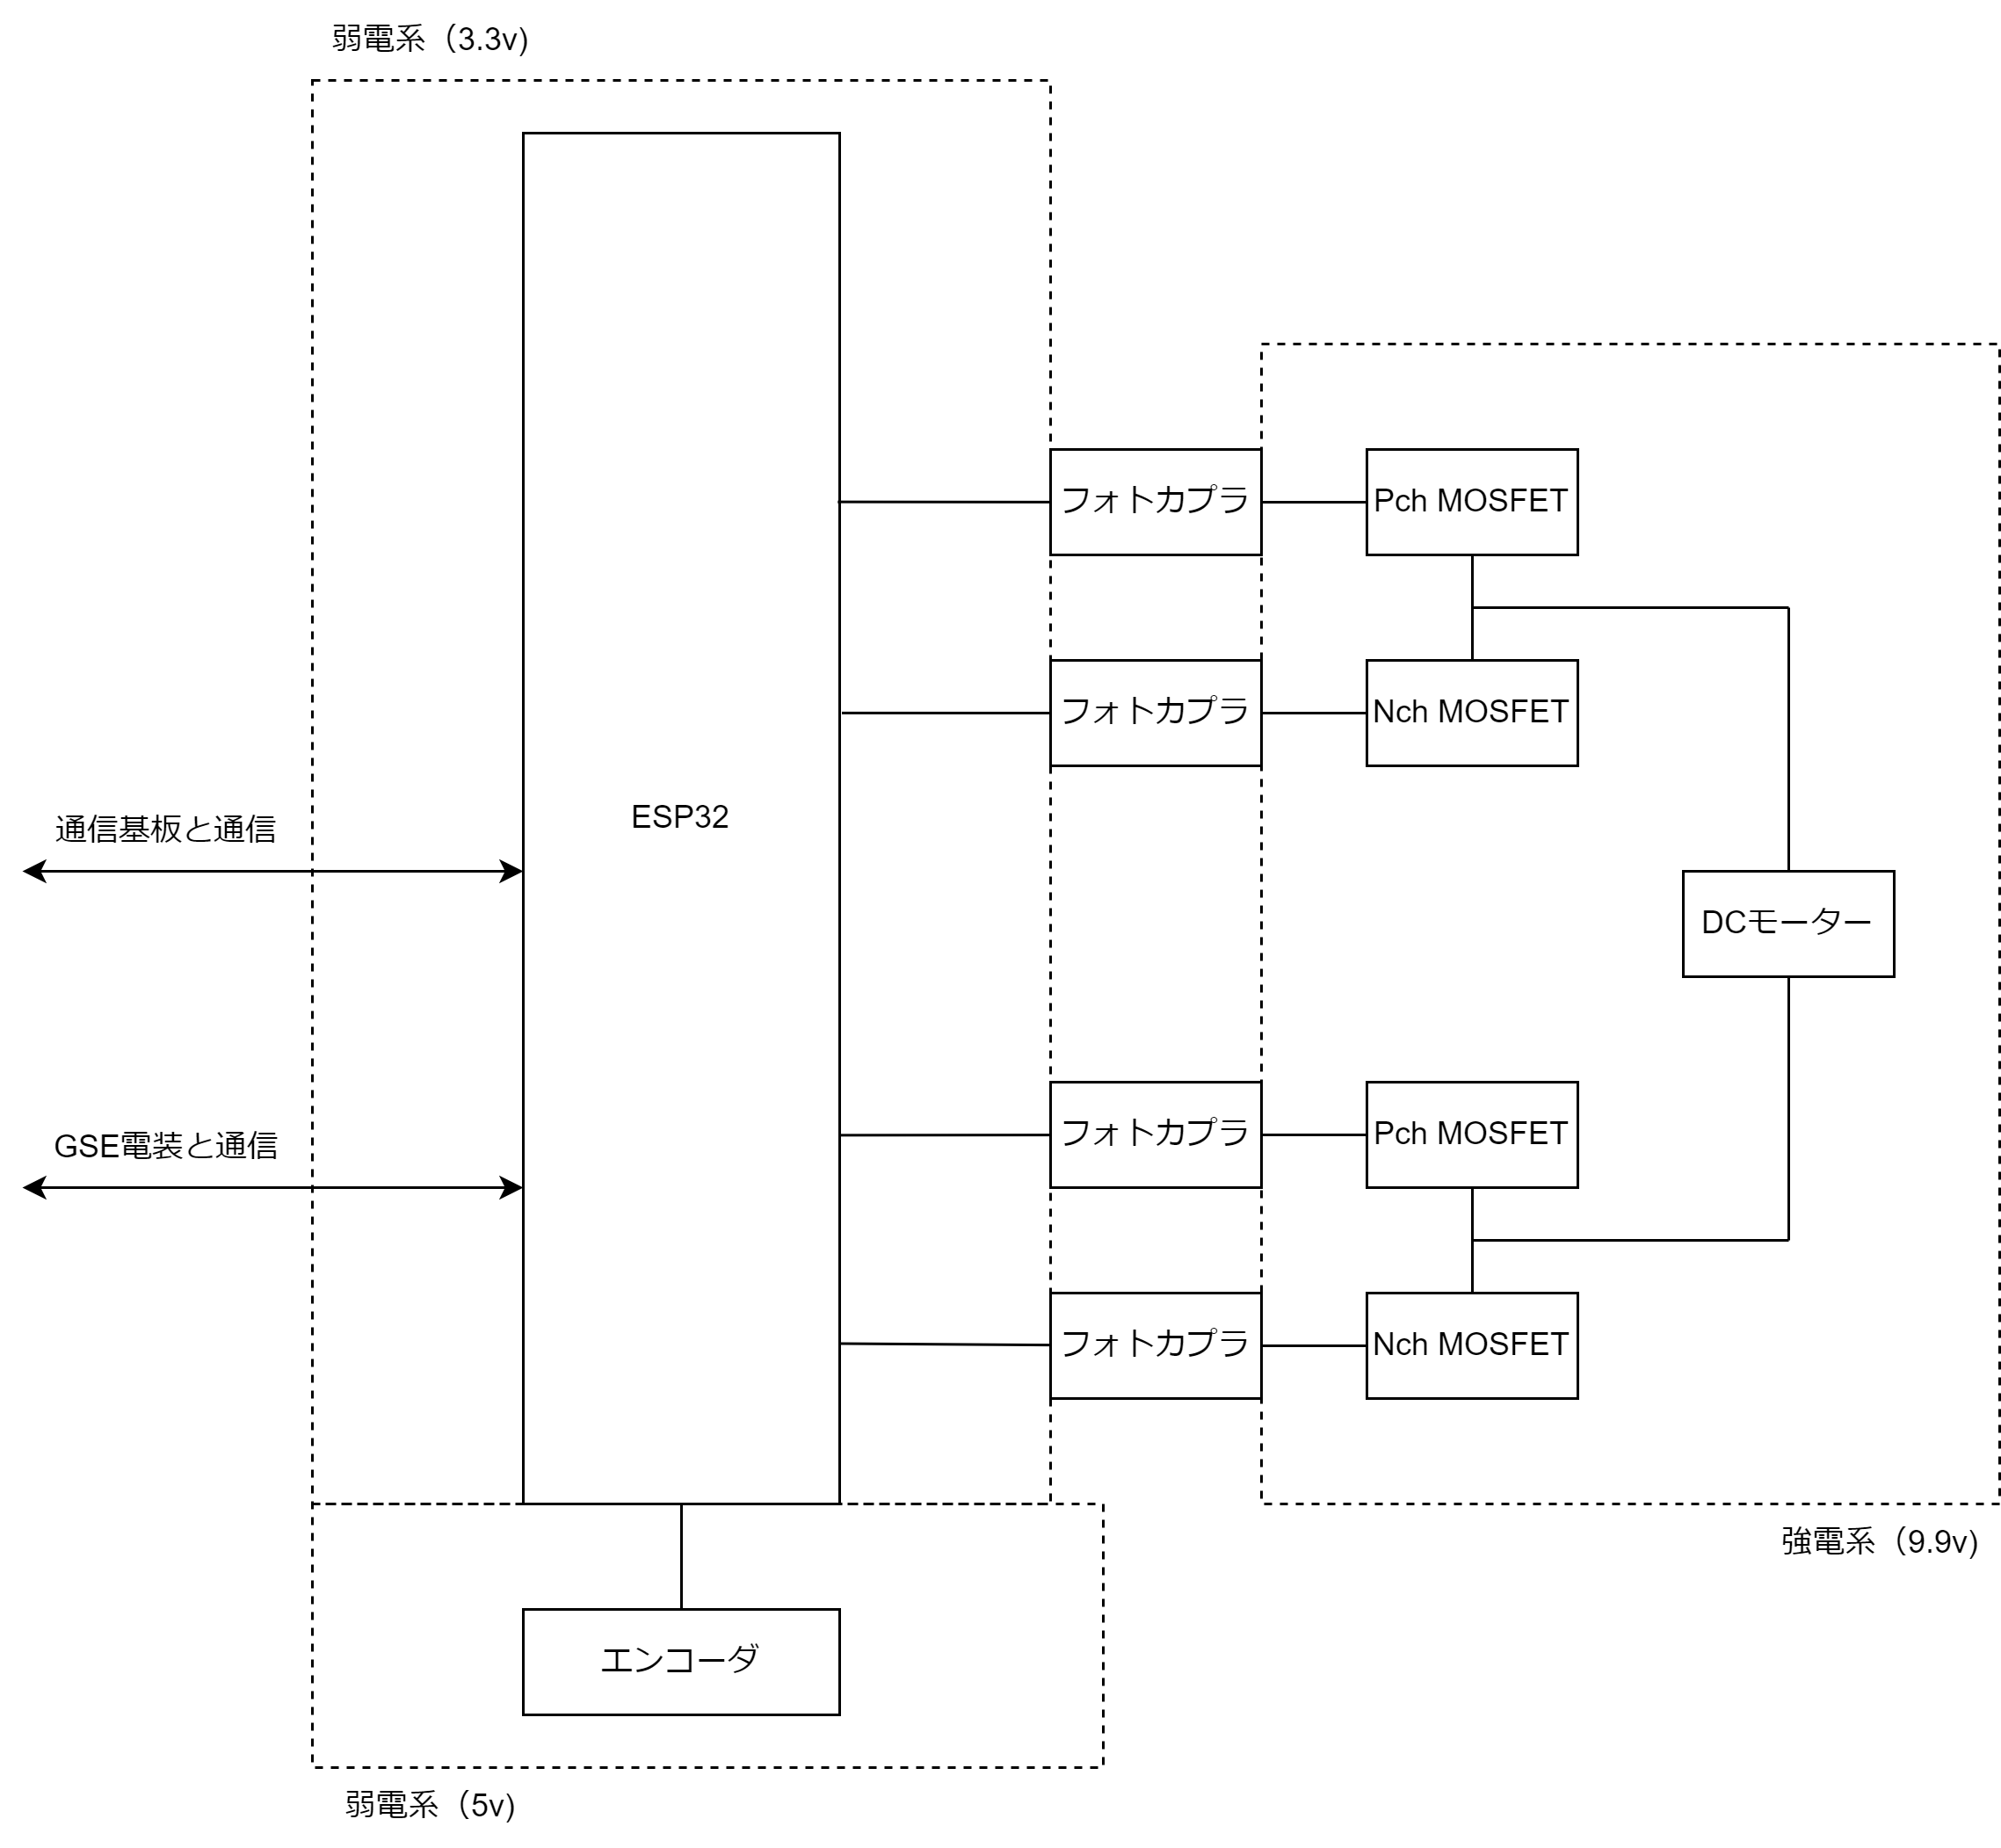
\includegraphics[width = 15cm]{figures/newGenPropulsionBRDChart.drawio.png}
    \caption{ロケット搭載基板のシステムチャート}
    \label{newGenPropulsionBRDChart}
\end{figure}

弱電系は制御、通信を行う電気系であり、マイクロコントローラはESP32を用いる。
強電系はDCモータを駆動する電気系であり、Pch MOSFETおよびNch MOSGETから構成されるHブリッジによってDCモータを駆動する。DCモーターはメインバルブの開閉に用いる。

強電系と弱電系の間の通信はフォトカプラによって絶縁される。

図\ref{powerSupplyChart}に本基板の電源構成図を示す。内部電源・外部電源がともに接続されている場合、ダイオードによって外部電源が選択され、内部電源からは電力が供給されないような設計である。

\begin{figure}[htbp]
    \centering
    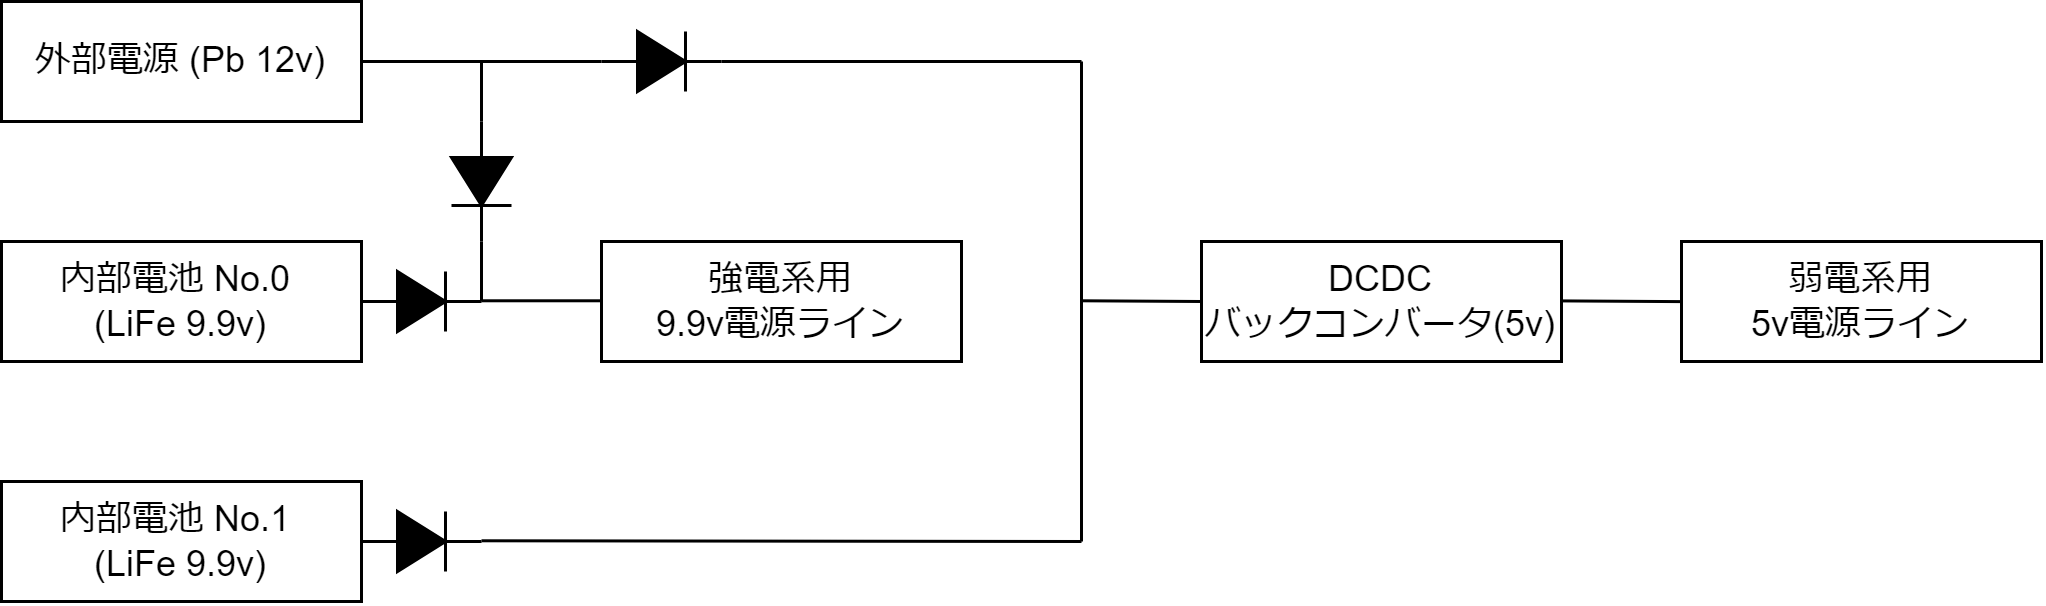
\includegraphics[width = 15cm]{figures/powerSupplyChart.drawio.png}
    \caption{ロケット搭載基板の電源構成図}
    \label{powerSupplyChart}
\end{figure}

表\ref{newGenPropulsionBRDPartList} に本基板における主要パーツを示す。

\begin{table}[htbp]
    \begin{tabular}{c|c|c}
        \hline
        ブロック名             & 型番                & 備考                                      \\ \hline \hline
        エンコーダ付きDCモータ & 備考参照            & \url{https://www.pololu.com/product/2828} \\ \hline
        Pch MOSFET             & MTB060P06I3         & 60V 16.7A                                 \\ \hline
        Nch MOSFET             & MTB30N06I3          & 60V 22A                                   \\ \hline
        フォトカプラ           & TLP785(GB F)        & Nch MOSFET(BSS138)を用いてドライブ        \\ \hline
        ESP32                  & ESP32-WROOM-32E-N16 &                                           \\
        \hline
    \end{tabular}
    \caption{ロケット搭載基板における主要搭載パーツ}
    \label{newGenPropulsionBRDPartList}
\end{table}


\subsection{GSE電装}

GSE電装のシステムチャートを図\ref{GSEAviChart} に示す。

\begin{figure}[htbp]
    \centering
    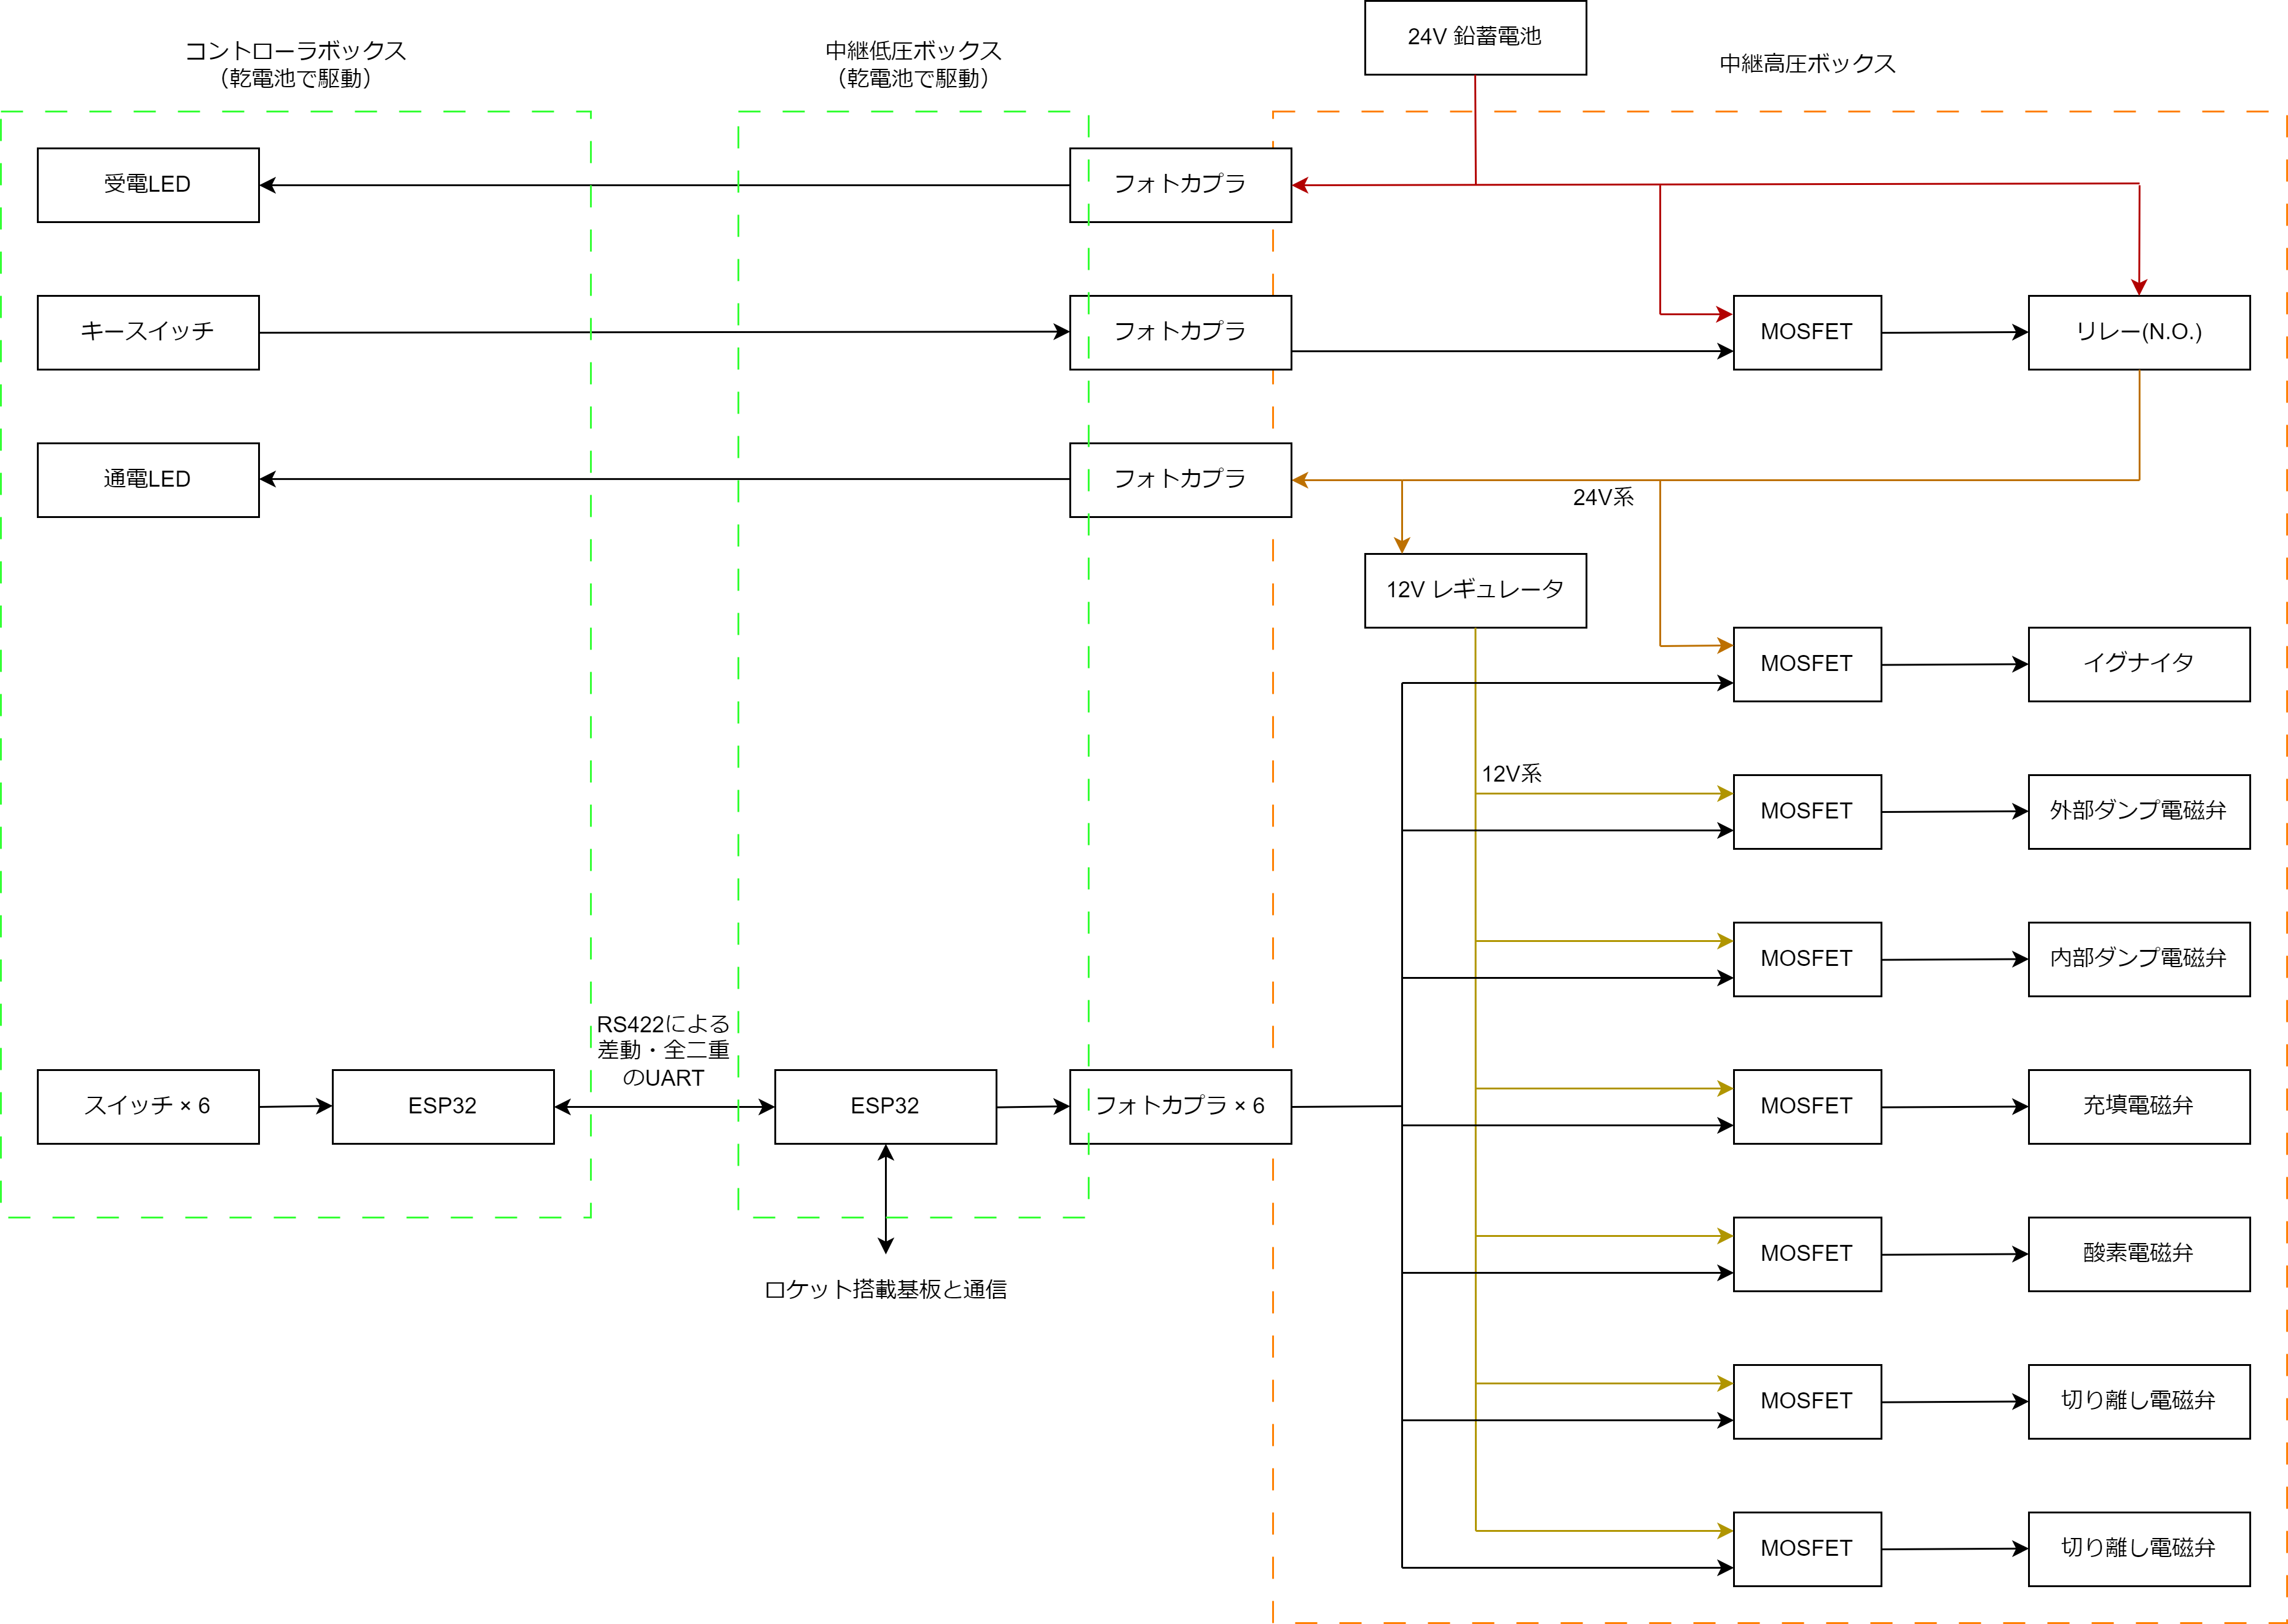
\includegraphics[width = 15cm]{figures/GSEAviChart.drawio.png}
    \caption{GSE電装のシステムチャート}
    \label{GSEAviChart}
\end{figure}

弱電系は制御、通信を行う電気系であり、マイクロコントローラはESP32を用いる。

強電系はイグナイタ・および電磁弁を駆動する電気系である。キースイッチをオンにすることで電源が投入され、キースイッチを抜くと電源が切れる設計である。

強電系と弱電系の間の通信はフォトカプラ・絶縁レギュレータによって絶縁される。

表\ref{GSEAviPartList} に本基板における主要パーツを示す。

\begin{table}[htbp]
    \begin{tabular}{c|c|c}
        \hline
        ブロック名           & 型番          & 備考                                                           \\ \hline \hline
        リレー               & G4A-1A-E DC24 & ノーマルオープン                                               \\ \hline
        12v レギュレータ     & NJM7812FA     & ヒートシンクを取り付けて使用                                   \\ \hline
        Nch MOSFET           & MTB30N06I3    & 60V 22A 電磁弁用、電磁弁の両極に保護のためダイオードを取付     \\ \hline
        Nch MOSFET           & TK5R3A06PL    & 60V 56A イグナイタ用、電磁弁の両極に保護のためダイオードを取付 \\ \hline
        フォトカプラ         & TLP785(GB F)  &                                                                \\ \hline
        絶縁レギュレータ(5v) & MAU105        &                                                                \\ \hline
        ESP32                & XIAO ESP32C3  &                                                                \\
        \hline
    \end{tabular}
    \caption{ロケット搭載基板における主要搭載パーツ}
    \label{GSEAviPartList}
\end{table}

\subsection{メインバルブ駆動用DCモータの制御について}

\subsection{点火シーケンス時の電装システムの動作について}


\end{document}